\documentclass[12pt]{article}
\usepackage{amsmath, amssymb, amsthm}
\usepackage{mathtools}
\usepackage{graphicx}
\usepackage{float}
\usepackage{hyperref}
\usepackage{xcolor}
\usepackage{listings}
\usepackage{geometry}
\usepackage{algorithm}
\usepackage{algpseudocode}
\usepackage{tikz}
\usepackage{longtable}
\usepackage{circuitikz}
\usepackage{comment}
\usepackage{MnSymbol}
\usepackage{physics}
\usepackage{booktabs}
\usepackage{subfig} % For \subfloat
\usepackage[section]{placeins}

\title{My Combined Document}
\author{Your Name}
\date{\today}

\begin{document}

\maketitle

\tableofcontents
\newpage

\section{Step Signal as $f(t)$}
For this analysis, we choose the \textbf{unit step function} as the input signal:

\begin{equation}
f(t) = u(t) = 
\begin{cases} 
1, & t \geq 0 \\
0, & t < 0 
\end{cases}
\end{equation}

\subsubsection{Interpretation:}
\begin{itemize}
    \item The output \( y(t) \) represents how the shape of \( f(t) \) is modified by \( h(t) \).
    \item The rectangular kernel \( h(t) \) acts as a moving average filter.
\end{itemize}

\subsection{Solution Using Step Function}

\subsubsection{Standard Convolution \( y(t) = (f * h)(t) \)}

Given:
\begin{itemize}
    \item \( f(t) = u(t) \) (step function)
    \item \( h(t) \) is a rectangular pulse centered at \( t = 0 \) with width \( 2T \).
\end{itemize}

The convolution integral is evaluated in three regions:

\begin{enumerate}
    \item \textbf{For \( t < -T \):}
    \begin{itemize}
        \item The kernel \( h(t - \tau) \) and \( u(\tau) \) do not overlap.
        \item Thus:
    \end{itemize}
    
    \begin{align}
        y(t) &= \int_{-\infty}^{\infty} u(\tau) h(t - \tau) \, d\tau \\
        &= \int_{0}^{\infty} 1 \cdot h(t - \tau) \, d\tau \\
        &= 0 \quad \text{(No overlap when $t < -T$)}
    \end{align}
    
    \item \textbf{For \( -T \leq t \leq T \):}
    \begin{itemize}
        \item The kernel partially overlaps \( u(\tau) \) from \( \tau = 0 \) to \( \tau = t + T \).
    \end{itemize}
    
    \begin{align}
        y(t) &= \int_{-\infty}^{\infty} u(\tau) h(t - \tau) \, d\tau \\
        &= \int_{0}^{\infty} 1 \cdot h(t - \tau) \, d\tau \\
        &= \int_{0}^{t+T} 1 \cdot 1 \, d\tau \quad \text{(Since $h(t-\tau)=1$ when $-T \leq t-\tau \leq T$)} \\
        &= [{\tau}]_{0}^{t+T} \\
        &= t + T
    \end{align}
    
    \item \textbf{For \( t > T \):}
    \begin{itemize}
        \item The kernel fully overlaps \( u(\tau) \) over a width of \( 2T \).
    \end{itemize}
    
    \begin{align}
        y(t) &= \int_{-\infty}^{\infty} u(\tau) h(t - \tau) \, d\tau \\
        &= \int_{0}^{\infty} 1 \cdot h(t - \tau) \, d\tau \\
        &= \int_{t-T}^{t+T} 1 \, d\tau \quad \text{(Since $h(t-\tau)=1$ when $t-T \leq \tau \leq t+T$)} \\
        &= [{\tau}]_{t-T}^{t+T} \\
        &= (t+T) - (t-T) \\
        &= 2T
    \end{align}
\end{enumerate}

\textbf{Final Result:}
\begin{equation}
y(t) = 
\begin{cases} 
0, & t < -T \\
t + T, & -T \leq t \leq T \\
2T, & t > T 
\end{cases}
\end{equation}

\subsubsection{Behavior Analysis:}
\begin{itemize}
    \item The output is zero before \( t = -T \).
    \item A linear ramp occurs from \( t = -T \) to \( t = T \).
    \item The output saturates at \( 2T \) for \( t > T \).
    \item A larger \( T \) results in a wider ramp and higher saturation value.
\end{itemize}
Here is plot showing the results
\begin{figure}[H]
    \centering
    \includegraphics[width=0.8\linewidth]{codes/codes_step/plotsstep/case1step.png}
    \label{fig:enter-label}
\end{figure}
\subsubsection{Modified Kernel (Only \( t > 0 \)) (Part a)}

The modified kernel is:
\begin{equation}
h_{mod}(t) = 
\begin{cases} 
1, & 0 \leq t \leq T \\
0, & \text{otherwise}
\end{cases}
\end{equation}

\textbf{Convolution Analysis:}

\begin{enumerate}
    \item \textbf{For \( t < 0 \):}
    \begin{align}
        y(t) &= \int_{-\infty}^{\infty} u(\tau) h_{mod}(t - \tau) \, d\tau \\
        &= 0 \quad \text{(No overlap when $t < 0$)}
    \end{align}
    
    \item \textbf{For \( 0 \leq t \leq T \):}
    \begin{align}
        y(t) &= \int_{-\infty}^{\infty} u(\tau) h_{mod}(t - \tau) \, d\tau \\
        &= \int_{0}^{t} 1 \cdot 1 \, d\tau \quad \text{(Overlap from $\tau = 0$ to $\tau = t$)} \\
        &= [{\tau}]_{0}^{t} \\
        &= t
    \end{align}
    
    \item \textbf{For \( t > T \):}
    \begin{align}
        y(t) &= \int_{-\infty}^{\infty} u(\tau) h_{mod}(t - \tau) \, d\tau \\
        &= \int_{t-T}^{t} 1 \cdot 1 \, d\tau \quad \text{(Full overlap from $\tau = t-T$ to $\tau = t$)} \\
        &= [{\tau}]_{t-T}^{t} \\
        &= t - (t-T) \\
        &= T
    \end{align}
\end{enumerate}

\textbf{Result:}
\begin{equation}
y(t) = 
\begin{cases} 
0, & t < 0 \\
t, & 0 \leq t \leq T \\
T, & t > T 
\end{cases}
\end{equation}
Here is a plot showing the results
\begin{figure}[H]
    \centering
    \includegraphics[width=0.8\linewidth]{codes/codes_step/plotsstep/case2step.png}
    \caption{Modified kernel}
    \label{fig:enter-label}
\end{figure}
\subsubsection{Comparison with Original Kernel:}
\begin{itemize}
    \item The response is now \textbf{causal} (output depends only on past/current inputs).
    \item The ramp is shorter (from \( 0 \) to \( T \)) compared to the original (\( -T \) to \( T \)).
    \item The steady-state value is \( T \) instead of \( 2T \).
\end{itemize}

\subsubsection{Shifted Kernel by \( \tau_0 \) (Part b)}

The shifted kernel is:
\begin{equation}
h_{shift}(t) = 
\begin{cases} 
1, & -T + \tau_0 \leq t \leq T + \tau_0 \\
0, & \text{otherwise}
\end{cases}
\end{equation}

Applying the time-shift property of convolution:
\begin{align}
f(t) * h(t-\tau_0) = (f(t) * h(t))_{t \rightarrow t-\tau_0}
\end{align}

The convolution output is simply the original \( y(t) \) delayed by \( \tau_0 \):

\begin{equation}
y_{shift}(t) = y(t - \tau_0) = 
\begin{cases} 
0, & t < -T + \tau_0 \\
(t - \tau_0) + T, & -T + \tau_0 \leq t \leq T + \tau_0 \\
2T, & t > T + \tau_0 
\end{cases}
\end{equation}
\begin{figure}[H]
    \centering
    \includegraphics[width=0.8\linewidth]{codes/codes_step/plotsstep/case3step.png}
    \caption{shifted kernel}
    \label{fig:enter-label}
\end{figure}

\subsubsection{Significance in Time-Delayed Systems:}
\begin{itemize}
    \item The shift \( \tau_0 \) introduces a \textbf{time delay} in the system's response.
    \item For \( \tau_0 > 0 \), the response is delayed (system responds later).
    \item For \( \tau_0 < 0 \), the response is advanced (system responds earlier).
    \item Important in control systems, signal processing, and communications where delays affect stability and synchronization.
\end{itemize}

\subsection{Conclusion}

\begin{itemize}
    \item The convolution of a step function with a rectangular kernel produces a \textbf{piecewise linear} output.
    \item Modifying the kernel to be \textbf{causal} changes the response to depend only on past inputs.
    \item Shifting the kernel introduces a \textbf{time delay}, which is crucial in real-world systems.
    \item The kernel width \( T \) directly affects the steady-state value and transition time of the output.
\end{itemize}

This analysis demonstrates how different kernel modifications affect signal processing outcomes and provides insight into the behavior of linear time-invariant systems.
\subsubsection{Comparision of all cases}
\begin{figure}[H]
    \centering
    \includegraphics[width=0.8\linewidth]{codes/codes_step/plotsstep/comparsionof123.png}
    \caption{Comparision of all cases}
    \label{fig:enter-label}
\end{figure}

\section*{1. Problem Statement}

\subsection*{1.1 Convolution with a Rectangular Kernel}
Compute the convolution of a given signal \( f(t) \) with a rectangular kernel \( h(t) \), analytically. The rectangular kernel is defined as:

\begin{equation}
h(t) = 
\begin{cases} 
1, & \text{for } -T \leq t \leq T \\
0, & \text{otherwise}
\end{cases}
\end{equation}

Derive the convolution expression \( y(t) = (f * h)(t) \) in terms of known functions, and analyze the system's behavior for various values of the kernel duration \( T \) and the input signal \( f(t) \).

Additionally, investigate the following scenarios:

\begin{enumerate}
    \item[(a)] Modify the kernel to only consider the part for \( t > 0 \). How does this affect the convolution result?
    \item[(b)] Shift the kernel by a time \( \tau_0 \). Analyze how the shift impacts the convolution output and discuss its significance in time-delayed systems.
\end{enumerate}

\textbf{Choice of Input Signal:}\\
For this analysis, we choose the \textbf{unit step function} as the input signal:

\begin{equation}
f(t) = u(t) = 
\begin{cases} 
1, & t \geq 0 \\
0, & t < 0 
\end{cases}
\end{equation}

\section*{2. Convolution Basics}

The convolution of two signals \( f(t) \) and \( h(t) \) is defined as:

\begin{equation}
y(t) = (f * h)(t) = \int_{-\infty}^{\infty} f(\tau) h(t - \tau) \, d\tau
\end{equation}

\subsection*{Interpretation:}
\begin{itemize}
    \item The output \( y(t) \) represents how the shape of \( f(t) \) is modified by \( h(t) \).
    \item The rectangular kernel \( h(t) \) acts as a moving average filter.
\end{itemize}

\section*{3. Solution Using Step Function}

\subsection*{3.1 Standard Convolution \( y(t) = (f * h)(t) \)}

Given:
\begin{itemize}
    \item \( f(t) = u(t) \) (step function)
    \item \( h(t) \) is a rectangular pulse centered at \( t = 0 \) with width \( 2T \).
\end{itemize}

The convolution integral is evaluated in three regions:

\begin{enumerate}
    \item \textbf{For \( t < -T \):}
    \begin{itemize}
        \item The kernel \( h(t - \tau) \) and \( u(\tau) \) do not overlap.
        \item Thus:
    \end{itemize}
    
    \begin{align}
        y(t) &= \int_{-\infty}^{\infty} u(\tau) h(t - \tau) \, d\tau \\
        &= \int_{0}^{\infty} 1 \cdot h(t - \tau) \, d\tau \\
        &= 0 \quad \text{(No overlap when $t < -T$)}
    \end{align}
    
    \item \textbf{For \( -T \leq t \leq T \):}
    \begin{itemize}
        \item The kernel partially overlaps \( u(\tau) \) from \( \tau = 0 \) to \( \tau = t + T \).
    \end{itemize}
    
    \begin{align}
        y(t) &= \int_{-\infty}^{\infty} u(\tau) h(t - \tau) \, d\tau \\
        &= \int_{0}^{\infty} 1 \cdot h(t - \tau) \, d\tau \\
        &= \int_{0}^{t+T} 1 \cdot 1 \, d\tau \quad \text{(Since $h(t-\tau)=1$ when $-T \leq t-\tau \leq T$)} \\
        &= [{\tau}]_{0}^{t+T} \\
        &= t + T
    \end{align}
    
    \item \textbf{For \( t > T \):}
    \begin{itemize}
        \item The kernel fully overlaps \( u(\tau) \) over a width of \( 2T \).
    \end{itemize}
    
    \begin{align}
        y(t) &= \int_{-\infty}^{\infty} u(\tau) h(t - \tau) \, d\tau \\
        &= \int_{0}^{\infty} 1 \cdot h(t - \tau) \, d\tau \\
        &= \int_{t-T}^{t+T} 1 \, d\tau \quad \text{(Since $h(t-\tau)=1$ when $t-T \leq \tau \leq t+T$)} \\
        &= [{\tau}]_{t-T}^{t+T} \\
        &= (t+T) - (t-T) \\
        &= 2T
    \end{align}
\end{enumerate}

\textbf{Final Result:}
\begin{equation}
y(t) = 
\begin{cases} 
0, & t < -T \\
t + T, & -T \leq t \leq T \\
2T, & t > T 
\end{cases}
\end{equation}

\subsection*{Behavior Analysis:}
\begin{itemize}
    \item The output is zero before \( t = -T \).
    \item A linear ramp occurs from \( t = -T \) to \( t = T \).
    \item The output saturates at \( 2T \) for \( t > T \).
    \item A larger \( T \) results in a wider ramp and higher saturation value.
\end{itemize}
Here is plot showing the results
\begin{figure}[H]
    \centering
    \includegraphics[width=0.8\linewidth]{plotsstep/case1step.png}
    \label{fig:enter-label}
\end{figure}
\subsection*{3.2 Modified Kernel (Only \( t > 0 \)) (Part a)}

The modified kernel is:
\begin{equation}
h_{mod}(t) = 
\begin{cases} 
1, & 0 \leq t \leq T \\
0, & \text{otherwise}
\end{cases}
\end{equation}

\textbf{Convolution Analysis:}

\begin{enumerate}
    \item \textbf{For \( t < 0 \):}
    \begin{align}
        y(t) &= \int_{-\infty}^{\infty} u(\tau) h_{mod}(t - \tau) \, d\tau \\
        &= 0 \quad \text{(No overlap when $t < 0$)}
    \end{align}
    
    \item \textbf{For \( 0 \leq t \leq T \):}
    \begin{align}
        y(t) &= \int_{-\infty}^{\infty} u(\tau) h_{mod}(t - \tau) \, d\tau \\
        &= \int_{0}^{t} 1 \cdot 1 \, d\tau \quad \text{(Overlap from $\tau = 0$ to $\tau = t$)} \\
        &= [{\tau}]_{0}^{t} \\
        &= t
    \end{align}
    
    \item \textbf{For \( t > T \):}
    \begin{align}
        y(t) &= \int_{-\infty}^{\infty} u(\tau) h_{mod}(t - \tau) \, d\tau \\
        &= \int_{t-T}^{t} 1 \cdot 1 \, d\tau \quad \text{(Full overlap from $\tau = t-T$ to $\tau = t$)} \\
        &= [{\tau}]_{t-T}^{t} \\
        &= t - (t-T) \\
        &= T
    \end{align}
\end{enumerate}

\textbf{Result:}
\begin{equation}
y(t) = 
\begin{cases} 
0, & t < 0 \\
t, & 0 \leq t \leq T \\
T, & t > T 
\end{cases}
\end{equation}
Here is a plot showing the results
\begin{figure}[H]
    \centering
    \includegraphics[width=0.8\linewidth]{plotsstep/case2step.png}
    \caption{Modified kernel}
    \label{fig:enter-label}
\end{figure}
\subsection*{Comparison with Original Kernel:}
\begin{itemize}
    \item The response is now \textbf{causal} (output depends only on past/current inputs).
    \item The ramp is shorter (from \( 0 \) to \( T \)) compared to the original (\( -T \) to \( T \)).
    \item The steady-state value is \( T \) instead of \( 2T \).
\end{itemize}

\subsection*{3.3 Shifted Kernel by \( \tau_0 \) (Part b)}

The shifted kernel is:
\begin{equation}
h_{shift}(t) = 
\begin{cases} 
1, & -T + \tau_0 \leq t \leq T + \tau_0 \\
0, & \text{otherwise}
\end{cases}
\end{equation}

Applying the time-shift property of convolution:
\begin{align}
f(t) * h(t-\tau_0) = (f(t) * h(t))_{t \rightarrow t-\tau_0}
\end{align}

The convolution output is simply the original \( y(t) \) delayed by \( \tau_0 \):

\begin{equation}
y_{shift}(t) = y(t - \tau_0) = 
\begin{cases} 
0, & t < -T + \tau_0 \\
(t - \tau_0) + T, & -T + \tau_0 \leq t \leq T + \tau_0 \\
2T, & t > T + \tau_0 
\end{cases}
\end{equation}
\begin{figure}[H]
    \centering
    \includegraphics[width=0.8\linewidth]{plotsstep/case3step.png}
    \caption{shifted kernel}
    \label{fig:enter-label}
\end{figure}
\subsection*{Significance in Time-Delayed Systems:}
\begin{itemize}
    \item The shift \( \tau_0 \) introduces a \textbf{time delay} in the system's response.
    \item For \( \tau_0 > 0 \), the response is delayed (system responds later).
    \item For \( \tau_0 < 0 \), the response is advanced (system responds earlier).
    \item Important in control systems, signal processing, and communications where delays affect stability and synchronization.
\end{itemize}

\section*{4. Conclusion}

\begin{itemize}
    \item The convolution of a step function with a rectangular kernel produces a \textbf{piecewise linear} output.
    \item Modifying the kernel to be \textbf{causal} changes the response to depend only on past inputs.
    \item Shifting the kernel introduces a \textbf{time delay}, which is crucial in real-world systems.
    \item The kernel width \( T \) directly affects the steady-state value and transition time of the output.
\end{itemize}

This analysis demonstrates how different kernel modifications affect signal processing outcomes and provides insight into the behavior of linear time-invariant systems.
\subsection*{Comparision of all cases}
\begin{figure}[H]
    \centering
    \includegraphics[width=0.8\linewidth]{plotsstep/comparsionof123.png}
    \caption{Comparision of all cases}
    \label{fig:enter-label}
\end{figure}

\section{Sinusoidal as $f(t)$ with Half-Box Kernel}

Compute the convolution of a given signal \( f(t) \) with a rectangular kernel \( h(t) \), analytically. The rectangular kernel is defined as:
\[
h(t) = 
\begin{cases}
1, & \text{for } -T \leq t \leq T, \\
0, & \text{otherwise}.
\end{cases}
\]
...

\subsection{Modify the kernel to only consider the part of the kernel for \( t > 0 \). How does this affect the convolution result?}

\subsubsection{Analytic}
In this analysis, we investigate the convolution of a sinusoidal input signal
\[
f(t) = A \sin(\omega t + \phi)
\]
with a rectangular kernel that is modified as below. The modified rectangular kernel is defined as:

\[
h(t) =
\begin{cases}
1, & \text{for } 0 < t < T, \\
0, & \text{otherwise}.
\end{cases}
\]

Our goal is to derive the convolution expression \( y(t) = (f \ast h)(t) \) analytically and analyze the system’s behavior.

The convolution of \( f(t) \) and \( h(t) \) is defined as:
\[
y(t) = (f \ast h)(t) = \int_{-\infty}^{\infty} f(\tau) h(t - \tau) \, d\tau
\]

Substituting our functions:
\[
y(t) = \int_{-\infty}^{\infty} A \sin(\omega \tau + \phi) \cdot h(t - \tau) \, d\tau
\]

Since the kernel \( h(t - \tau) \) is non-zero only when \( 0  < t - \tau <  T \), we can rewrite this condition as:
\[
t - T < \tau < t
\]

Therefore, the limits of integration become:
\[
y(t) = \int_{t - T}^{t} A \sin(\omega \tau + \phi) \, d\tau
\]

Evaluating this integral:
The integral of \( \sin(\omega \tau + \phi) \) is:
\[
\int \sin(\omega \tau + \phi) \, d\tau = -\frac{1}{\omega} \cos(\omega \tau + \phi)
\]

Evaluating the integral from \( t - T \) to \( t \):
\[
y(t) = A \left[ -\frac{1}{\omega} \cos(\omega \tau + \phi) \right]_{t - T}^{t}
\]

This simplifies to:
\[
y(t) = A \left( -\frac{1}{\omega} \cos(\omega t + \phi) + \frac{1}{\omega} \cos(\omega (t - T) + \phi) \right)
\]
Using the identity for the difference of cosines:
\[
\cos A - \cos B = -2 \sin\left( \frac{A + B}{2} \right) \sin\left( \frac{A - B}{2} \right)
\]
\[
y(t) = \frac{A}{\omega} \left( -2 \sin \left( \frac{(\omega (t - T) + \phi) + (\omega t + \phi)}{2} \right) \sin \left( \frac{(\omega (t - T) + \phi) - (\omega t + \phi)}{2} \right) \right)
\]
\[
y(t) = \frac{A}{\omega} \left( -2 \sin \left( \omega t + \phi - \frac{\omega T}{2} \right) \sin \left( \frac{\omega T}{2} \right) \right)
\]
\[
\boxed{y(t) = \frac{2A \sin\left( \frac{\omega T}{2} \right)}{\omega} \sin \left( \omega( t  - \frac{T}{2}) + \phi \right)}
\]
The convolution for the modified kernel does not change the behavior of the signal, i.e., the output still remains sinusoidal.The significant differences are as follows :
\begin{itemize}
\item A $ \frac{T}{2} $ time shift towards right .

\item The scaling of amplitude is changed from $\frac{2\sin(\omega T)}{\omega}$ to $\frac{2\sin(\frac{\omega T}{2})}{\omega}$ .
\end{itemize}

\begin{figure}
    \centering
    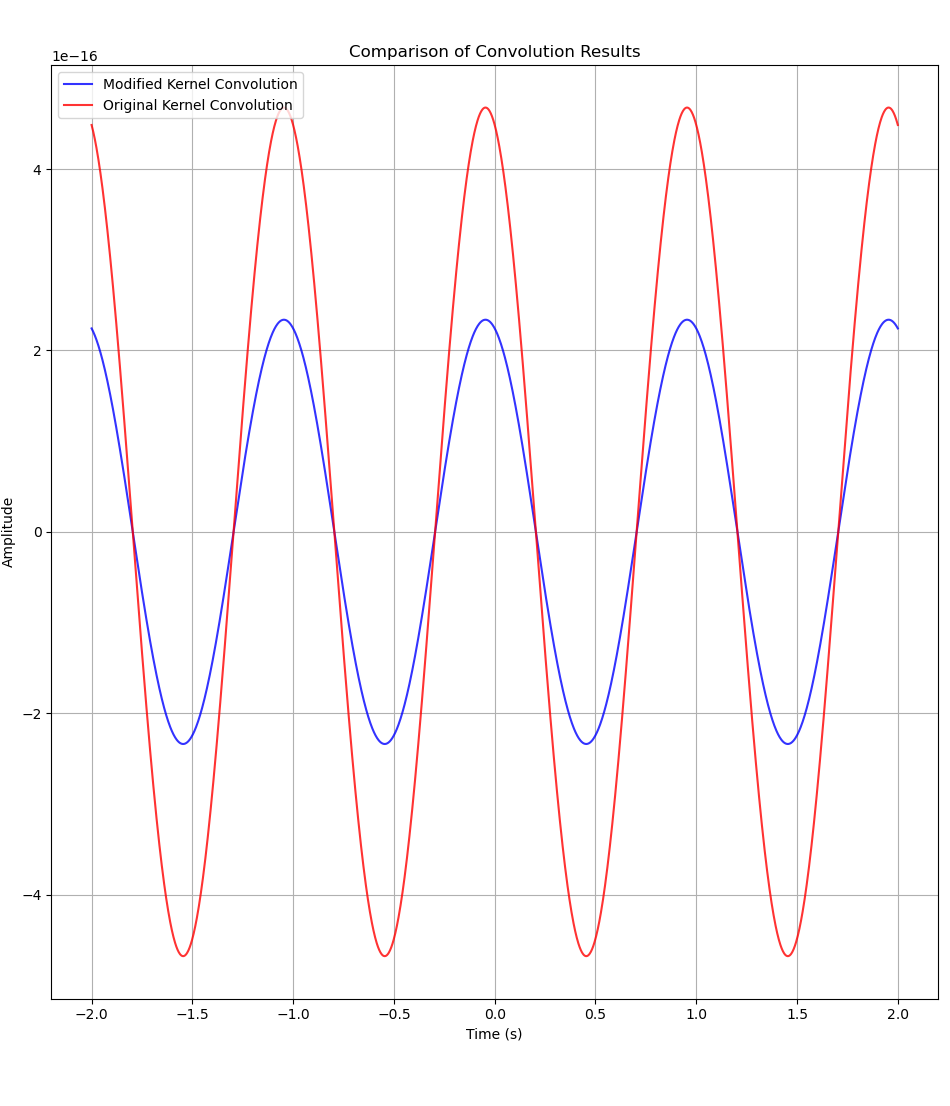
\includegraphics[width=0.5\linewidth]{codes/codes_sin_2/figs/compare.png}
    \caption{Plot of the convolutions}
    \label{fig:enter-label}
\end{figure}

\newpage

\subsection{Extended Graphical and Analytical Analysis}

\subsubsection{Effect of Amplitude \( A \)}

The first figure below demonstrates the impact of changing amplitude values on the convolution result. As seen, increasing the amplitude scales the overall magnitude of the output signal, keeping the shape unchanged.
\begin{figure}[h]
    \centering
    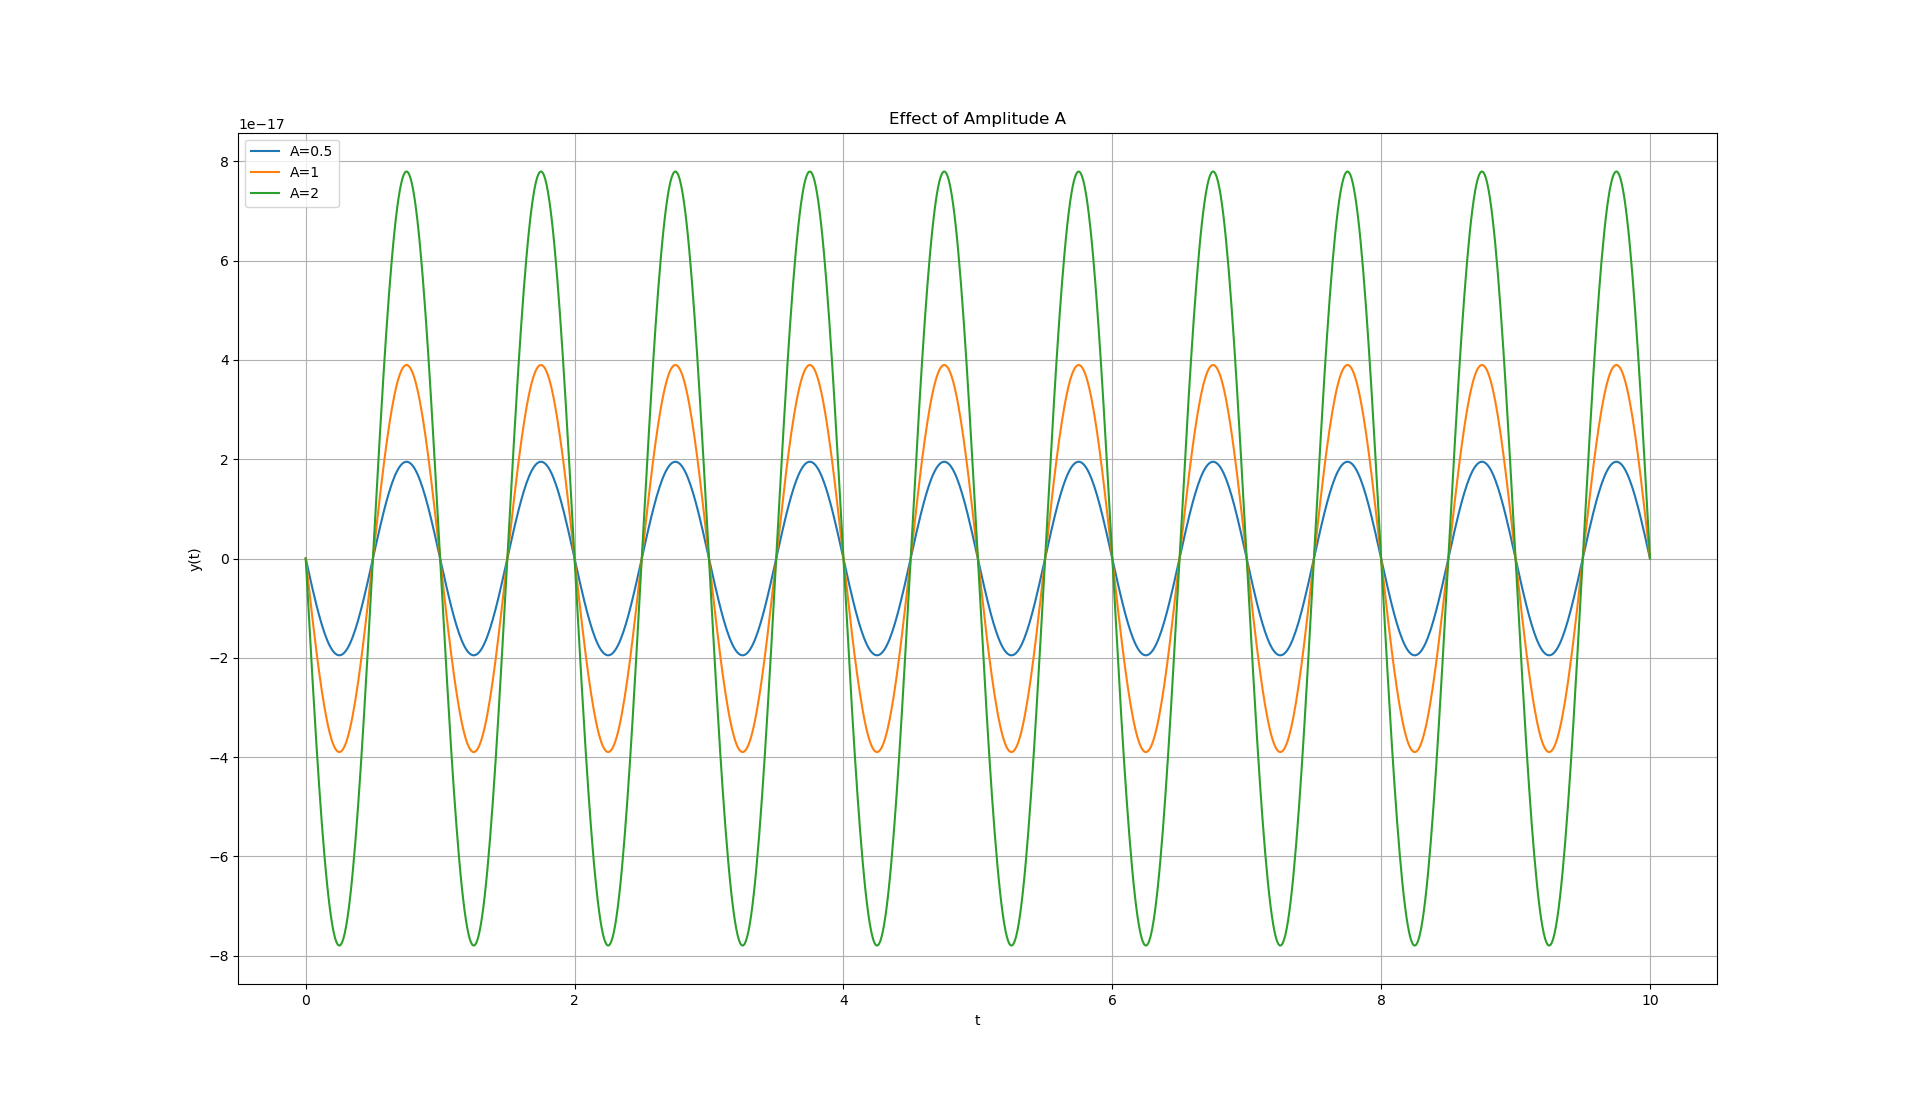
\includegraphics[width=0.8\textwidth]{codes/codes_sin_2/figs/amp.png}
    \caption{Effect of varying amplitude \( A \) on the convolution output.}
\end{figure}



\subsubsection{Effect of Angular Frequency \( \omega \)}

Changing \( \omega \) changes how rapidly the sinusoidal input oscillates. This figure shows how higher frequencies start diminishing in magnitude due to the sinc-type attenuation from the convolution.
\begin{figure}[h]
    \centering
    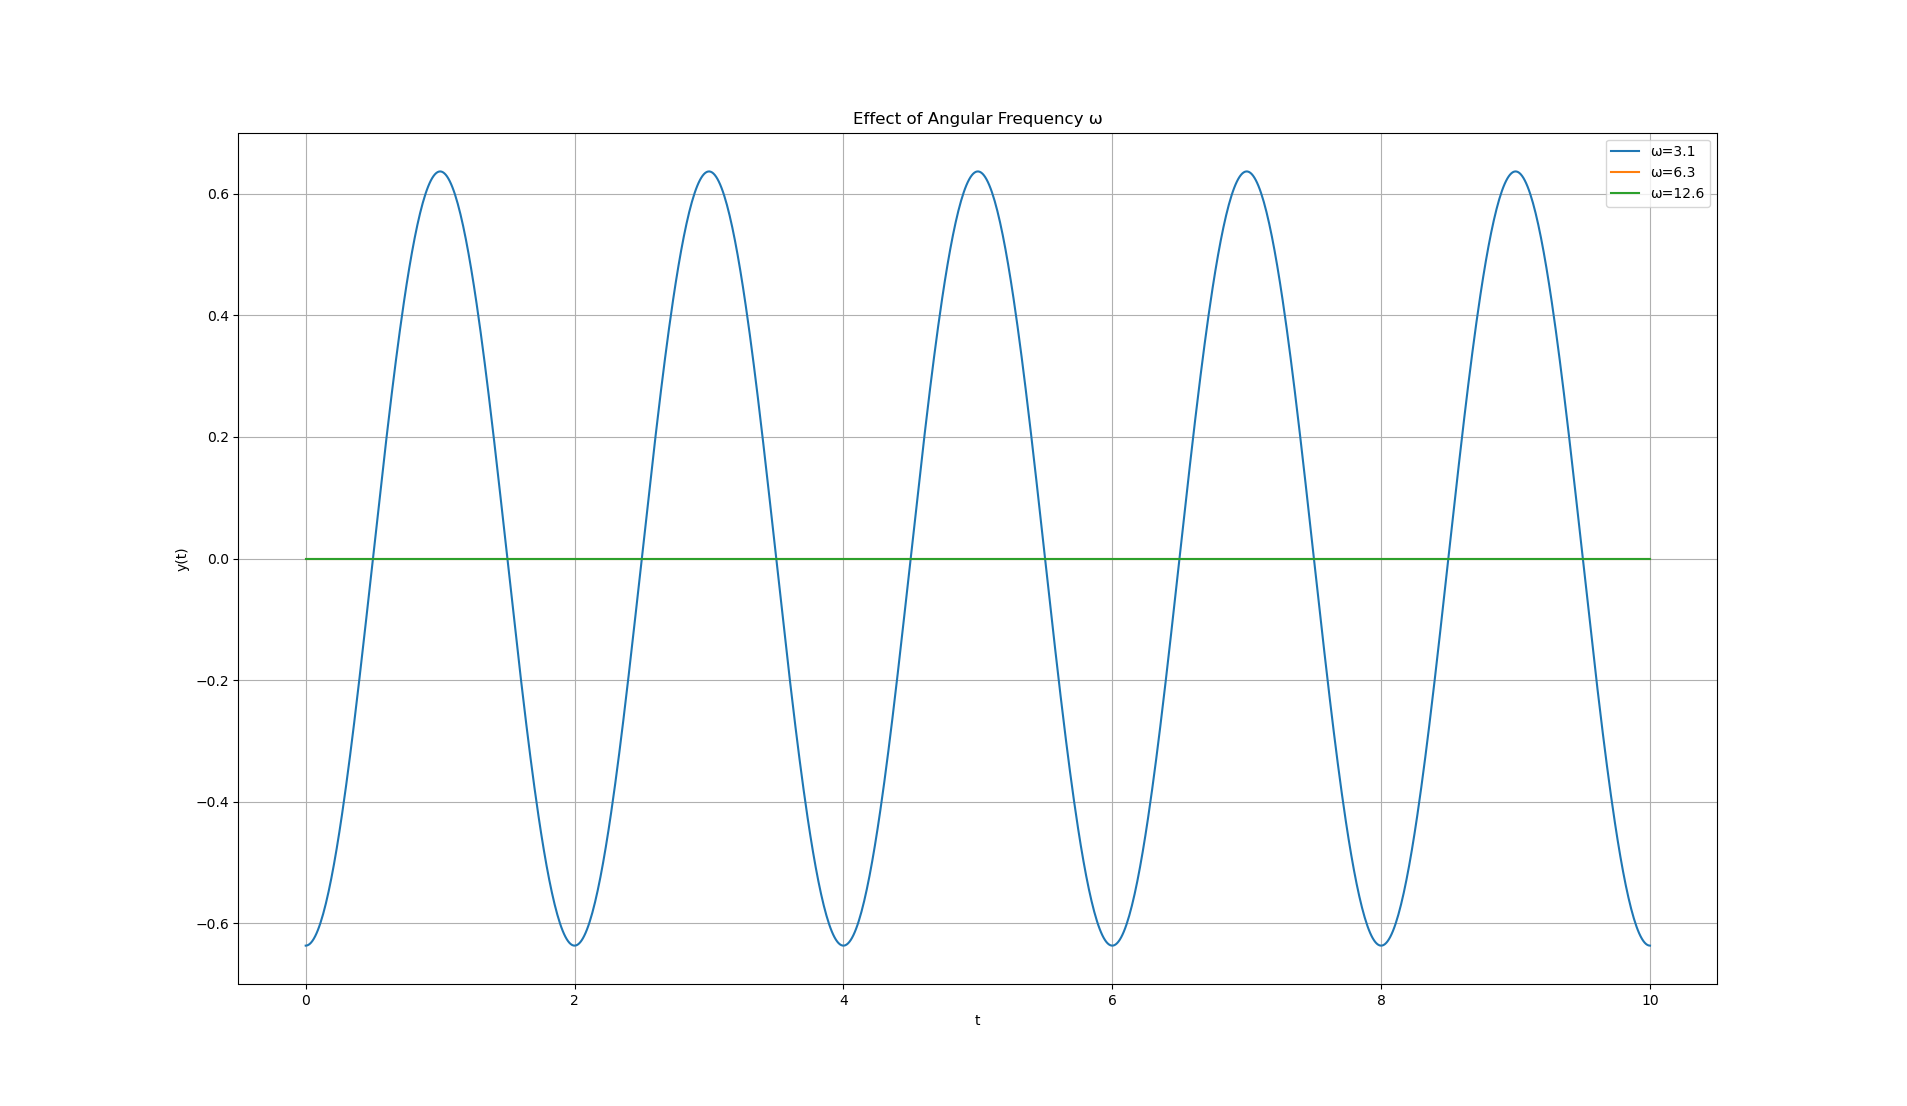
\includegraphics[width=0.8\textwidth]{codes/codes_sin_2/figs/omega.png}
    \caption{Effect of angular frequency \( \omega \) on convolution. Higher frequencies are attenuated.}
\end{figure}

\subsubsection{Effect of Pulse Width \( T \)}

This graph demonstrates how varying \( T \), the width of the rectangular kernel, influences the output. Smaller \( T \) leads to lesser averaging, preserving high-frequency content. Larger \( T \) results in more smoothing.
\begin{figure}[h]
    \centering
    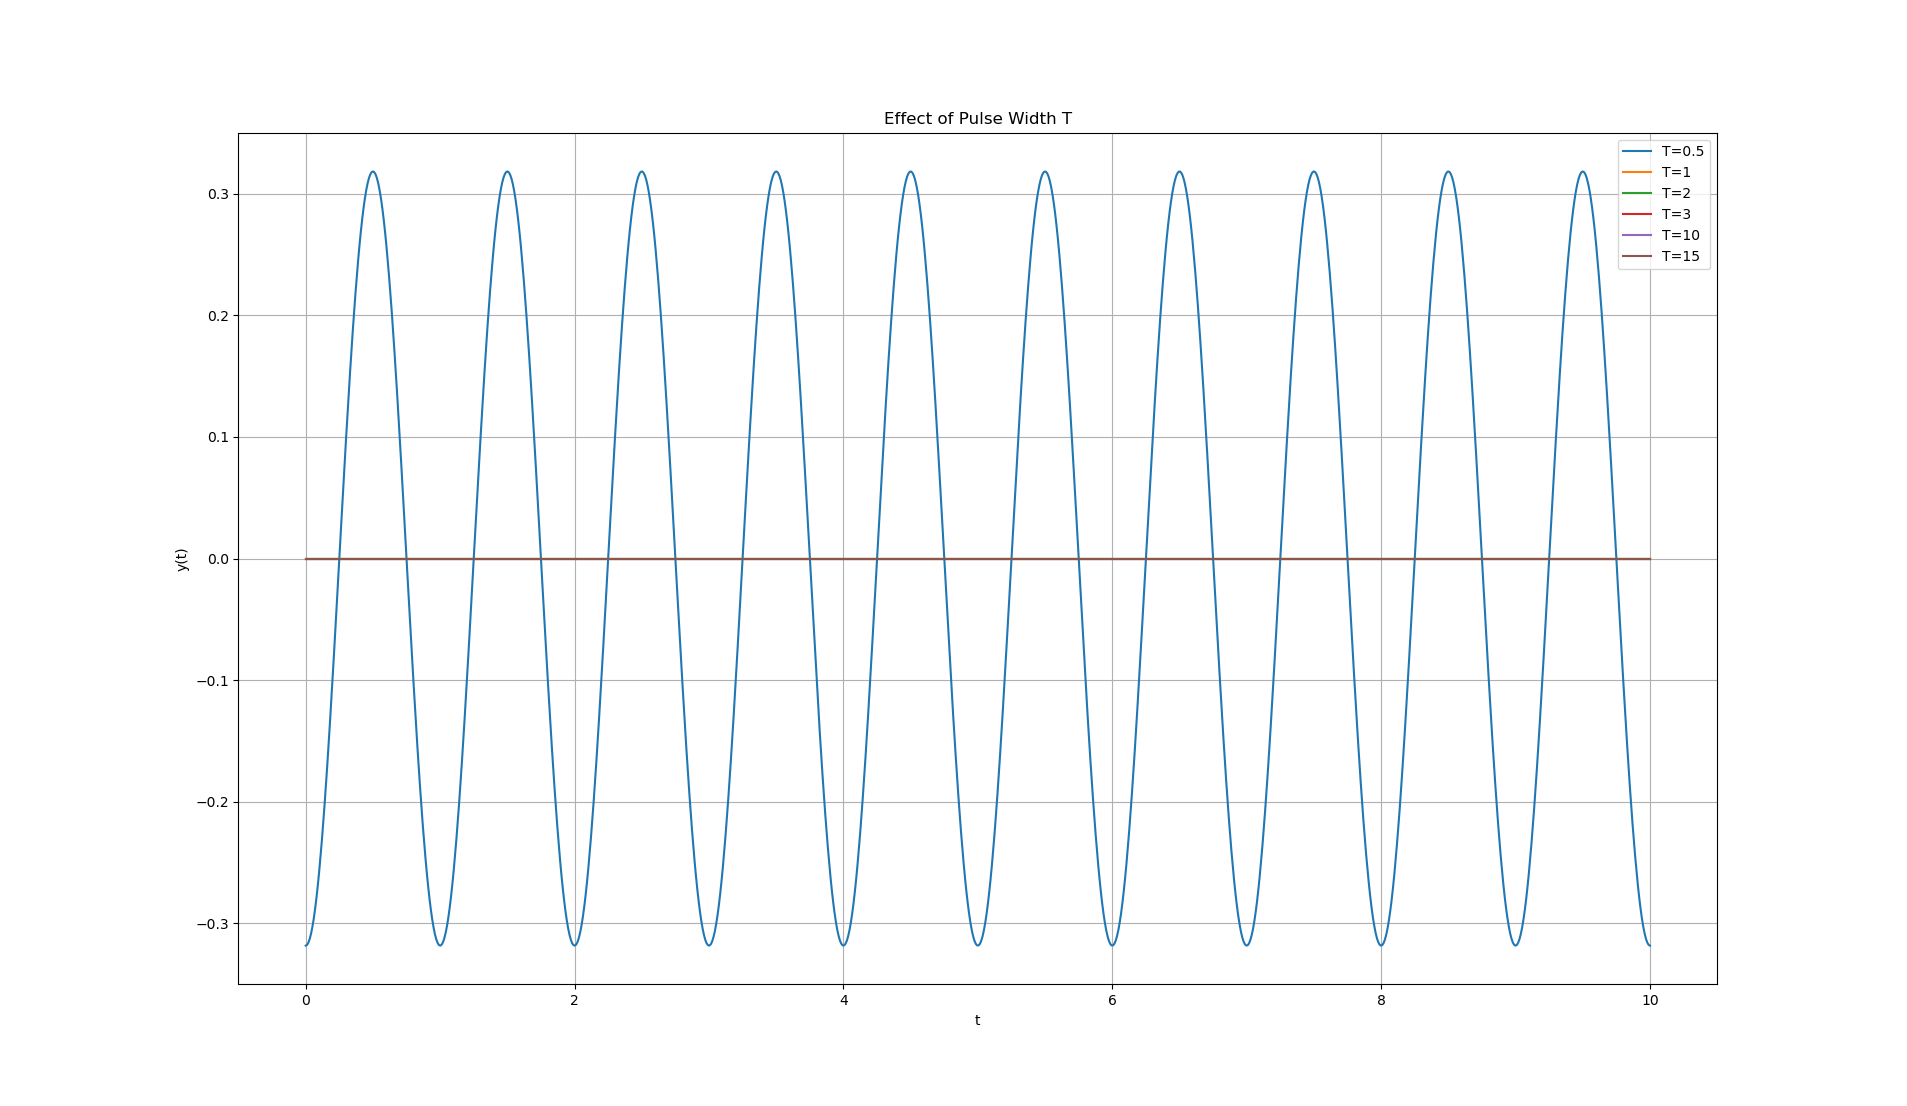
\includegraphics[width=0.8\textwidth]{codes/codes_sin_2/figs/T.png}
    \caption{Convolution output for different pulse widths \( T \).}
\end{figure}

\subsubsection{Amplitude Ratio vs Angular Frequency}

This plot captures the normalized amplitude ratio \( \frac{A_{out}}{A} = \frac{2\sin(\omega \frac{T}{2})}{\omega} \) as a function of \( \omega \) for various values of \( T \). It reflects the sinc-function behavior, emphasizing low-pass characteristics of convolution with rectangular kernels.
\begin{figure}[h]
    \centering
    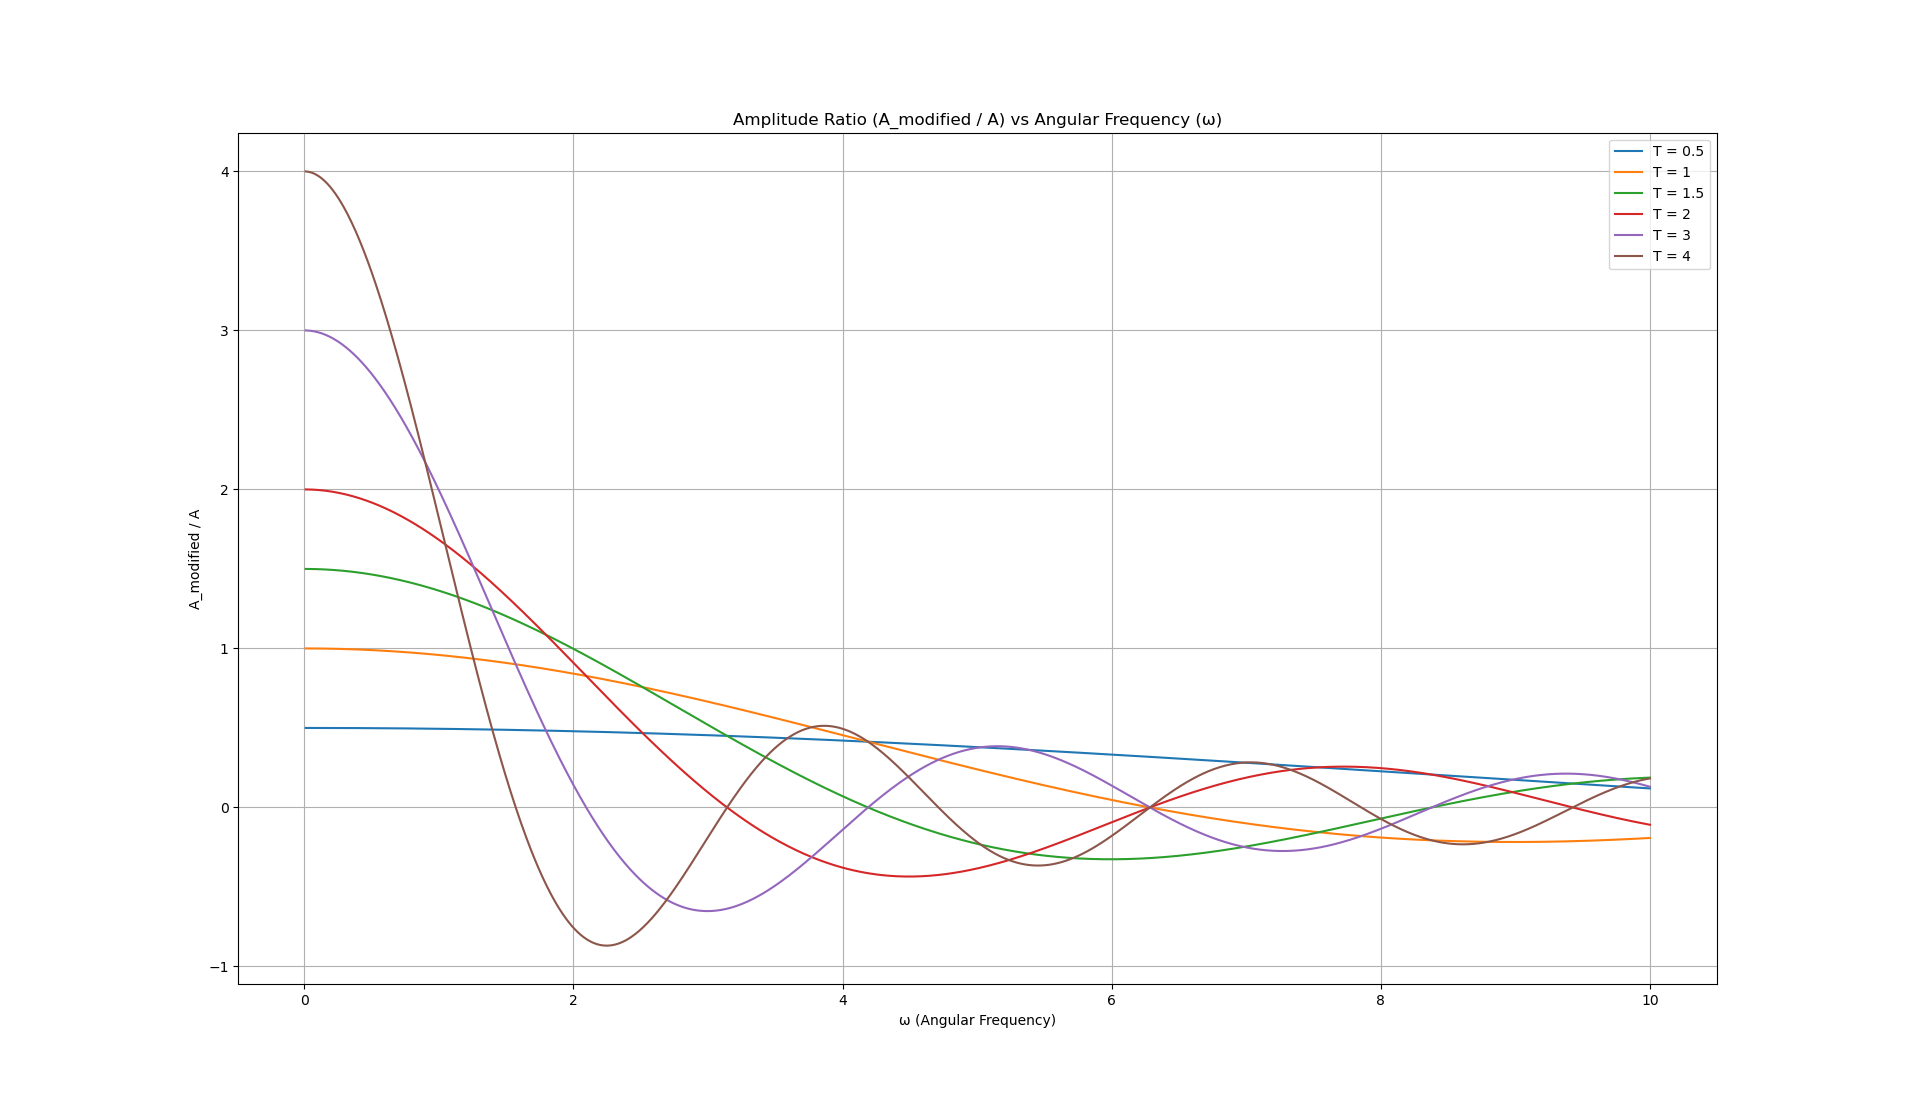
\includegraphics[width=0.8\textwidth]{codes/codes_sin_2/figs/scaling.png}
    \caption{Amplitude ratio \( \frac{A_{\text{modified}}}{A} \) versus angular frequency \( \omega \) for different values of \( T \).}
\end{figure}

\subsubsection{Effect of Phase \( \phi \)}

Altering the phase \( \phi \) of the sinusoidal signal results in horizontal shifts in the waveform. The output retains its shape but is delayed or advanced in time.
\begin{figure}[h]
    \centering
    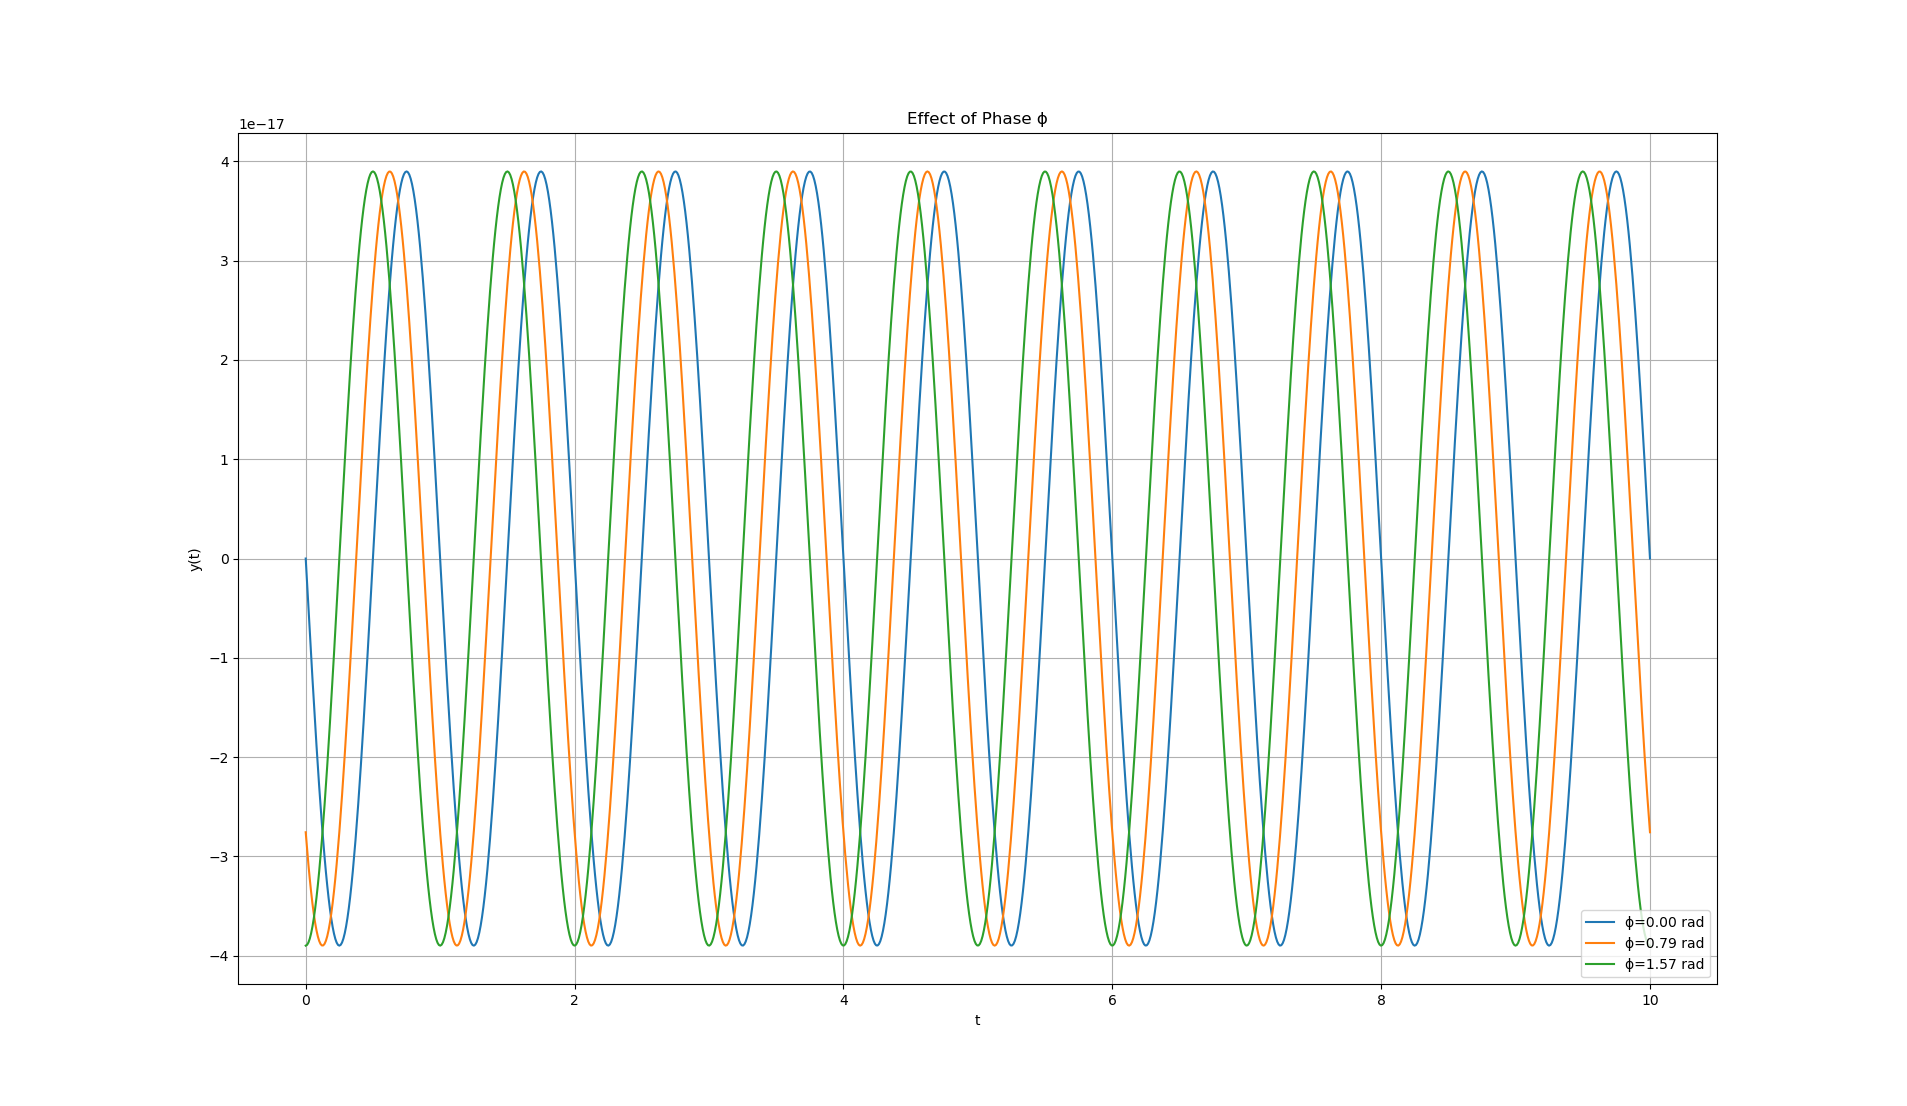
\includegraphics[width=0.8\textwidth]{codes/codes_sin_2/figs/phi.png}
    \caption{Phase shift \( \phi \) changes the horizontal alignment of the output signal.}
\end{figure}

\subsubsection{Special Observations}
\begin{itemize}
    \item If \( \omega T = n\pi \), the output vanishes, indicating frequency nulls.
    \item For large \( T \), the kernel acts as a low-pass filter.
    \item When \( T \rightarrow 0 \), the kernel approximates an impulse, and the convolution result tends to zero everywhere.
\end{itemize}

\subsection{Convolution with Varying Parameters}

The figure below shows the convolution output for multiple combinations of parameters including amplitude \( A \), frequency \( \omega \), kernel width \( T \), and phase \( \phi \). It highlights how these parameters influence the shape, scaling, and shift of the output signal.

Each sub-plot or curve within the figure corresponds to a unique configuration. You can observe:
\begin{itemize}
    \item Changes in amplitude due to scaling by \( \frac{2\sin(\omega T)}{\omega} \)
    \item Phase shifts resulting from both the signal phase \( \phi \) and kernel delay \( \tau_0 \)
    \item Smoothing effects due to increasing kernel width \( T \)
    \item Attenuation of high-frequency components, emphasizing the low-pass filter nature of box kernels
\end{itemize}

\begin{figure}[h]
    \centering
    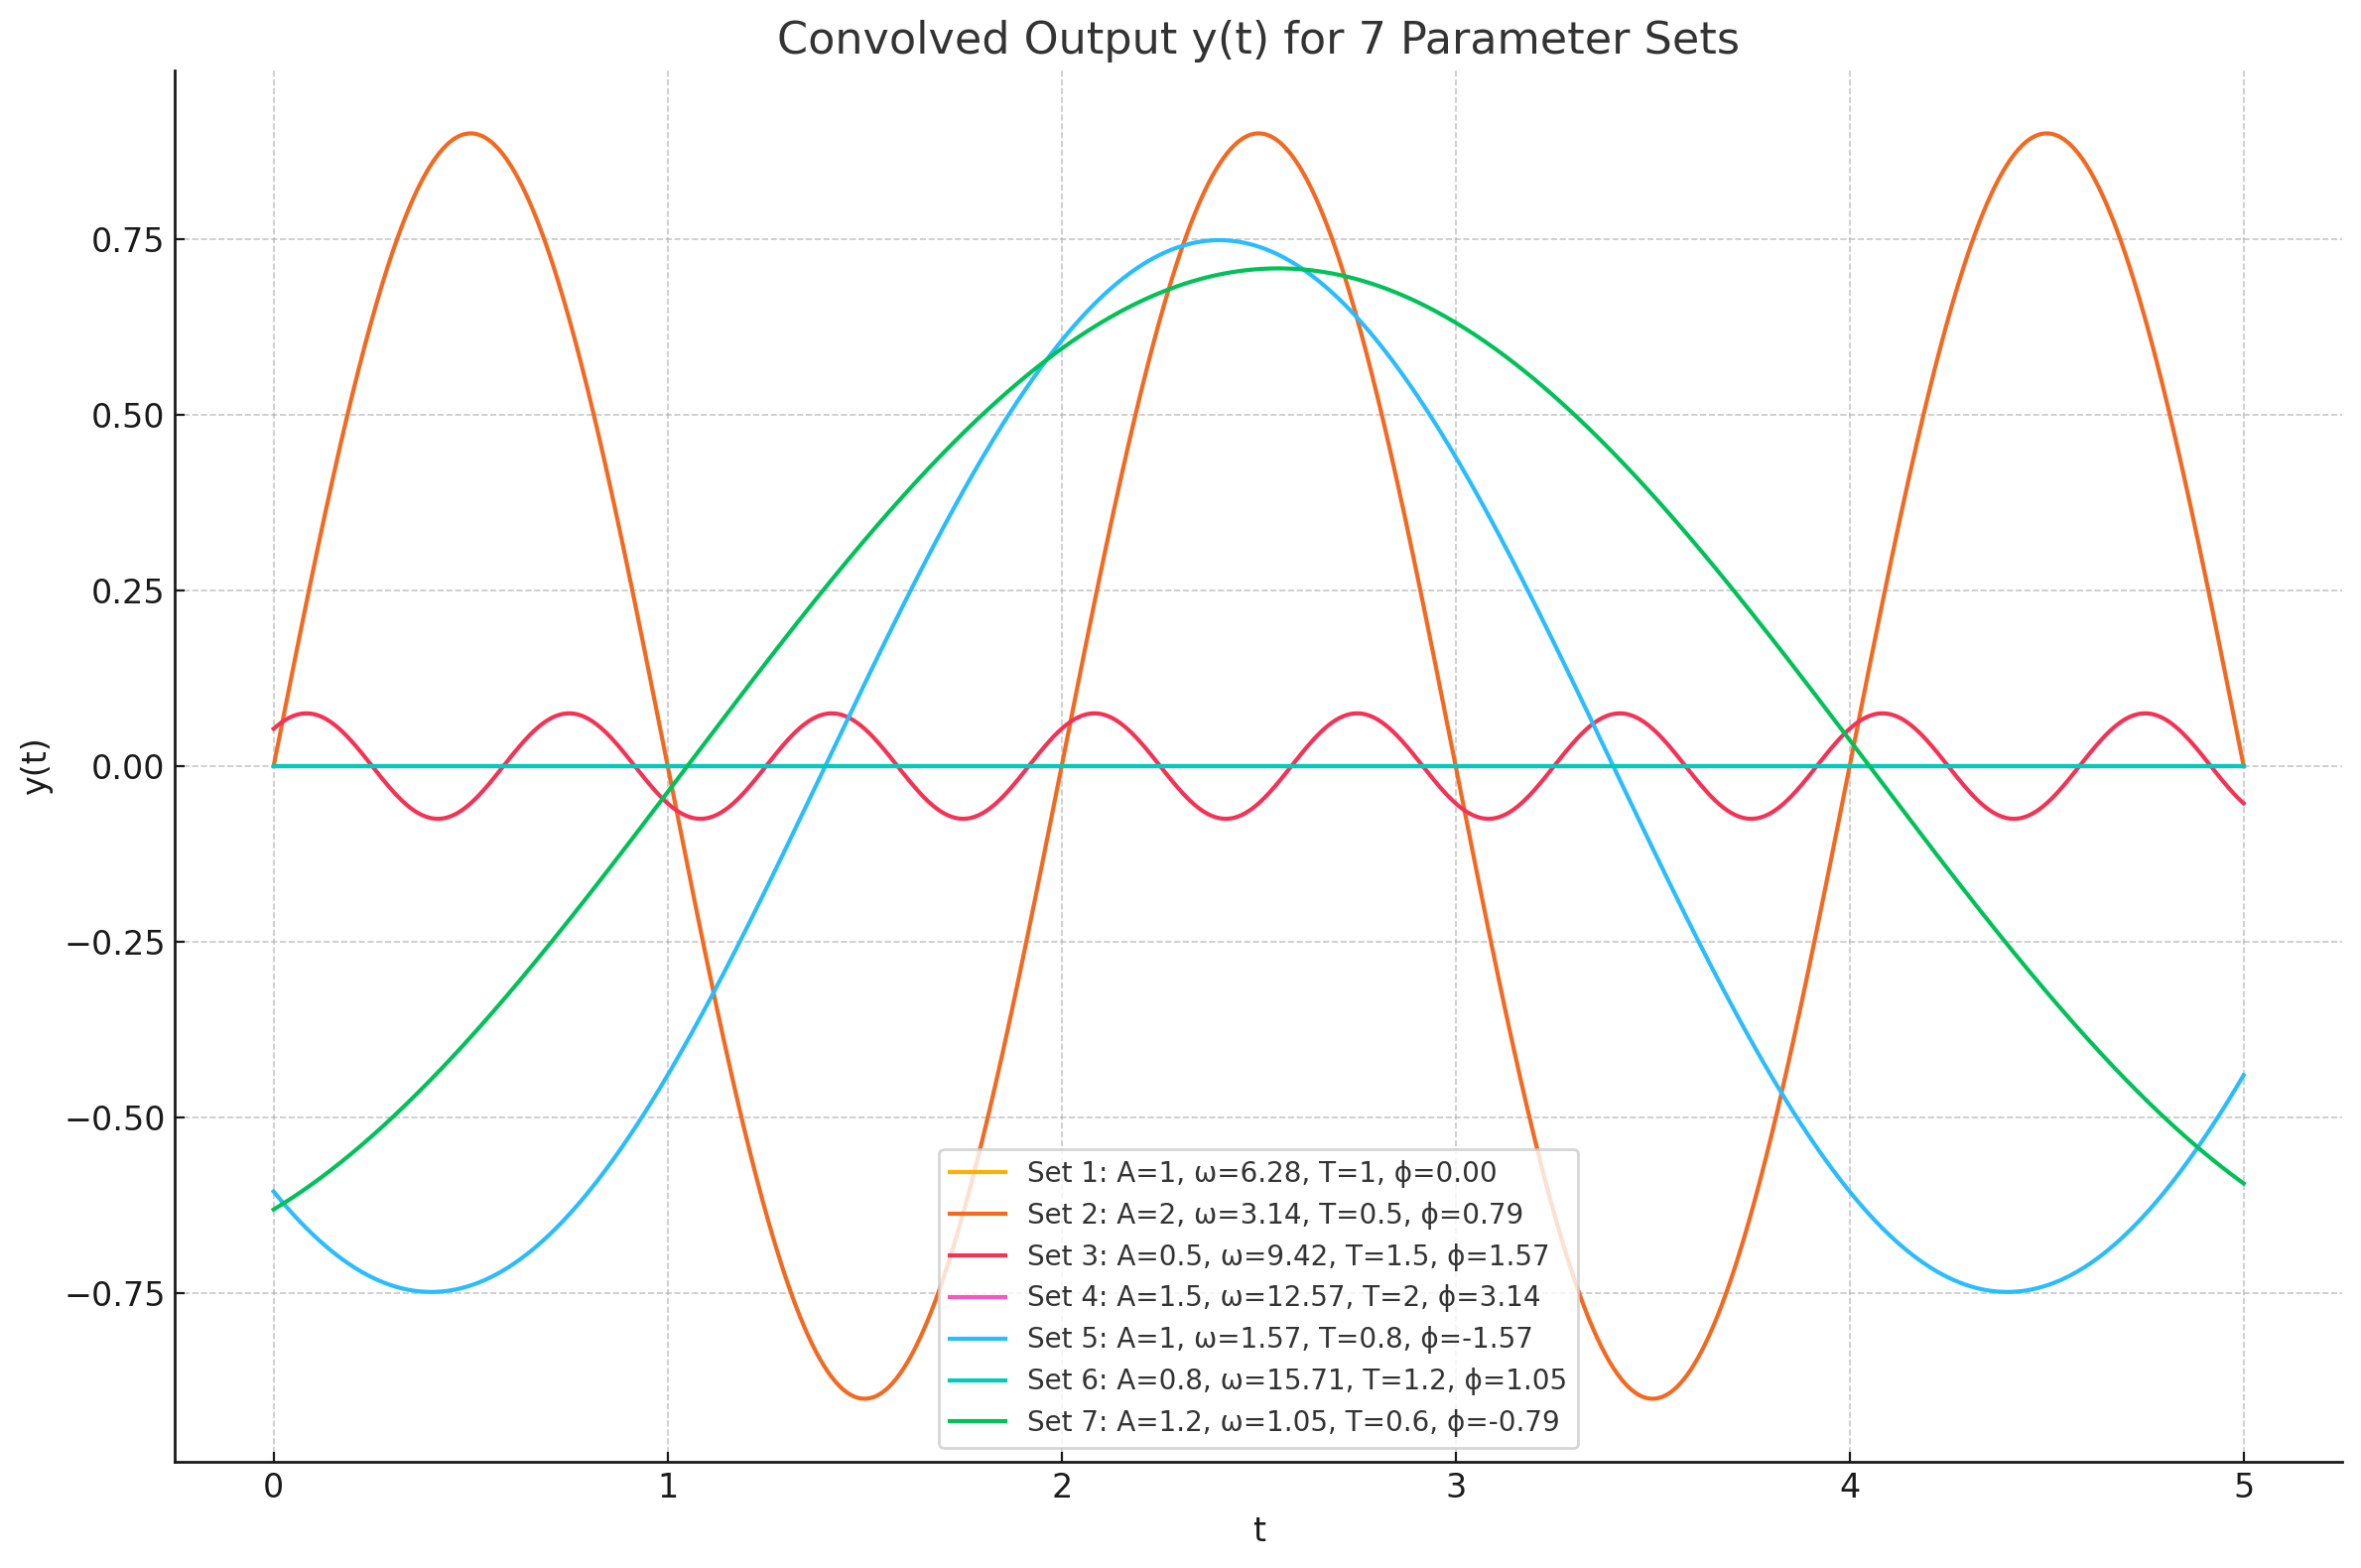
\includegraphics[width=0.7\textwidth]{codes/codes_sin_2/figs/all_varies.png}
    \caption{Convolution output for different parameter sets \( (A, \omega, T, \phi) \).}
\end{figure}


\subsection{Conclusion}

This detailed analysis of convolution using a rectangular kernel shows how parameters such as amplitude, frequency, kernel width, and phase influence the output signal. The kernel acts as a smoothing and low-pass filter, selectively attenuating high-frequency components. Additionally, time-shifting the kernel leads to equivalent shifts in the output, demonstrating important system properties like linearity and time invariance.

\end{document}


\end{document}
